% Construction : droite graduée, centre a = 2.6, rayon r = 1.4.
%   L'intervalle [a - r ; a + r] = [1.2 ; 4] est le segment épais.
%   Les deux flèches marquent la distance r de part et d'autre de a.
% SVG : x = 30 + 52x, y = 74 (axe).
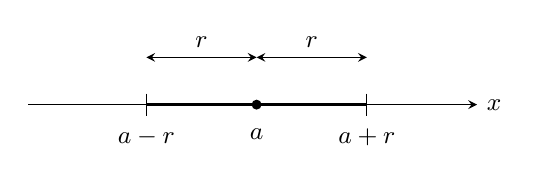
\begin{tikzpicture}[scale=1, >=stealth, every node/.style={font=\small}]
  \draw[->] (-0.3, 0) -- (5.4, 0) node[right] {$x$};
  \draw[very thick] (1.2, 0) -- (4, 0);
  \draw (1.2, 0.14) -- (1.2, -0.14); \draw (4, 0.14) -- (4, -0.14);
  \fill (2.6, 0) circle (1.8pt);
  \draw[<->] (1.2, 0.6) -- (2.6, 0.6) node[midway, above] {$r$};
  \draw[<->] (2.6, 0.6) -- (4, 0.6) node[midway, above] {$r$};
  \node[below] at (2.6, -0.18) {$a$};
  \node[below] at (1.2, -0.18) {$a - r$};
  \node[below] at (4, -0.18) {$a + r$};
\end{tikzpicture}
